\documentclass{beamer}
\usepackage{geometry}
\usepackage{amsmath}
\usepackage{amssymb}
\usepackage{graphicx}
\usepackage{hyperref}
\usepackage{fancyhdr}

\usetheme[mylogo]{Boadilla}

\title{The Reconstruction of Isengard}
\subtitle{The Design, Implementation, and Testing of a Bastion Host}
\author{Alex Hurd and Eric Richter}
\institute[COSI]{Clarkson Open Source Institute}

\hypersetup{
    bookmarks=true,         % show bookmarks bar?
    unicode=false,          % non-Latin characters in Acrobats bookmarks
    pdftoolbar=true,        % show Acrobats toolbar?
    pdfmenubar=true,        % show Acrobats menu?
    pdffitwindow=true,      % page fit to window when opened
    pdftitle={Lab 8},    % title
    pdfauthor={Alex Hurd and Eric Richter},     % author
    pdfsubject={Network Security},   % subject of the document
    pdfnewwindow=true,      % links in new window
    pdfkeywords={keywords}, % list of keywords
    colorlinks=true,       % false: boxed links; true: colored links
    linkcolor=blue,          % color of internal links
    citecolor=blue,        % color of links to bibliography
    filecolor=magenta,      % color of file links
    urlcolor=blue           % color of external links
}


%  \includegraphics[width=\textwidth]{SEZR.png}
\begin{document}

\begin{frame}
  \titlepage
\end{frame}

\begin{frame}
  \frametitle{Topics}
  \begin{enumerate}
    \item Bastion Host
    \item Network Monitoring/Firewall/Routing ``HyperCube''
    \item CS Lab Network Reconfiguration
    \item Implemented Security Policies
  \end{enumerate}
\end{frame}

\begin{frame}
  \frametitle{Bastion Host}
What is a Bastion Host?
  \begin{itemize}
    \item Bridge between internal network and outside world
    \item Elevated security
  \end{itemize}
  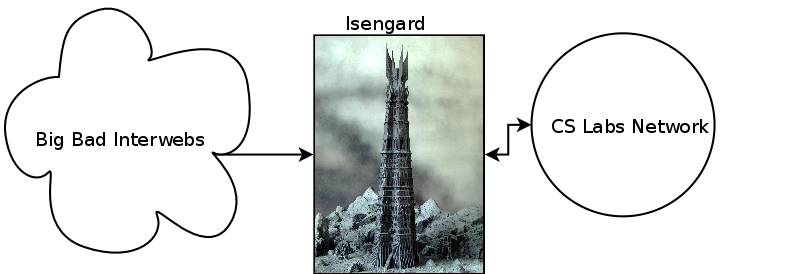
\includegraphics[width=\textwidth]{diagrams/isengard.png}
\end{frame}

\begin{frame}
  \frametitle{Bastion Host (cont.)}
Why is a Bastion Host important?
  \begin{itemize}
	\item Extra security (Obviously!)
    \item Monitoring/Accountability
    \item First layer of attacks from the outside 
  \end{itemize}
What goes behind the Bastion Host? (i.e. what goes through it?)
  \begin{itemize}
    \item All external SSH Traffic. This includes:
    \begin{itemize}
      \item Internal Services
      \item Web Hosts
      \item Student Projects
      \item ...and so on
    \end{itemize} 
  \end{itemize}
\end{frame}

\begin{frame}
  \frametitle{``HyperCube''}
What is the Network Monitoring/Firewalling/Routing Box?
  \begin{itemize}
    \item Intermediary between ALL traffic in and out of the network
    \item Traffic monitoring
    \item Act as a stateful firewall
    \item Have the capabilities to perform deep pack inspection
  \end{itemize}
Why is this ``HyperCube'' important?
  \begin{itemize}
    \item More security
    \item Pinpoint network abnormalities
    \item Provide usage statistics
  \end{itemize}
\end{frame}

\begin{frame}
  \frametitle{Network Reconfiguration}
EXPLAIN WHY WE NEED TO RECONFIGURE HERE
\end{frame}

\begin{frame}
  \frametitle{Network Reconfiguration (cont.)}
128.153.144 $\implies$ Inaccessible from Outside
  \begin{itemize}
    \item COSI/ITL Lab Machines
    \item Wireless Network
    \item Open Ethernet Ports
  \end{itemize}
128.153.145 $\implies$ SSH through Isengard
  \begin{itemize}
    \item Internal Services
  \end{itemize}
128.153.146 $\implies$ SSH from Clarkson, everything else open
  \begin{itemize}
    \item Web Hosts
    \item Student Projects
  \end{itemize}
\end{frame}

\begin{frame}
  \frametitle{Network Reconfiguration (tl;dr)} 
  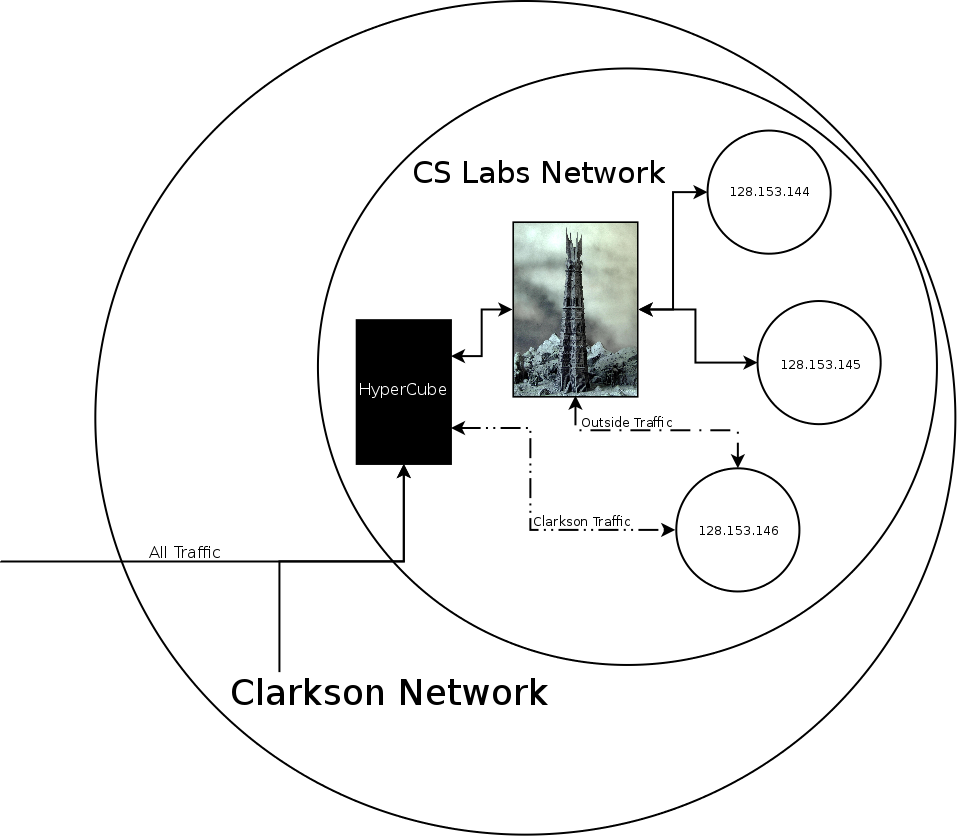
\includegraphics[height=\textheight]{diagrams/network.png}
\end{frame}

\begin{frame}
  \frametitle{Network Reconfiguration (cont.)}
Security Policies
  \begin{itemize}
      \item Europa \& Juno: Enforce SSH traffic only from Isengard
      \item Titan: Enforce SSH traffic from only Clarkson's Network (including Isengard)
  \end{itemize}
\end{frame}


\end{document} 
